\usetikzlibrary{shapes, arrows}
\usetikzlibrary{positioning}
\usetikzlibrary{shapes.geometric, arrows, positioning}
\usetikzlibrary{intersections, patterns, calc}

\tikzstyle{startstop} = [rectangle, rounded corners, minimum width=2cm, minimum height=1cm, text centered, draw=black]
\tikzstyle{process} = [rectangle, minimum width=2cm, minimum height=1cm, text centered, draw=black]
\tikzstyle{decision} = [diamond, minimum width=2cm, minimum height=1cm, text centered, draw=black]
\tikzstyle{arrow} = [thick,->,>=stealth]

\chapter{Generowanie modeli PL z~opisów tekstowych zagadnień optymalizacyjnych}\label{ch:generation}

\section{Wstęp teoretyczny}

% TP: Po co to? Przecież nie rozwiązujecie modeli PL, ani nie korzystacie w żaden sposób z tych twierdzeń; one też nie pasują do ogólniejszej klasy -> MILP, którą Wasza metoda obsługuje

% TP: TODO: Tutaj też sugeruję nie rozwodzić się nad zapisami, które są istotne z punktu widzenia metod rozwiązywania modeli PL; z punktu widzenia modelowania rozróżnienie postaci ogólnej i standardowej nie ma większego znaczenia. Z drugiej strony brakuje definicji modelu PL takiego, który Wy generujecie. 
% Dlatego sugeruję tutaj wprowadzić 3 sekcje:
% - Model Programowania Liniowego - tutaj definicja, która jest zgodna z reprezentacją ZIMPL
% - Problem generowania modelu PL z opisu tekstowego - tutaj poza formalnym postawieniem problemu należy omówić właściwości tego problemu; zdefiniujcie też warianty problem z parametryzacją i bez parametryzacji
% - Problem oceny modelu PL na zgodność z opisem tekstowym - formalny opis problemu i jego właściwości
% W załączeniu do maila dołączam przykładową pracę mgr, w której autor definiuje model PL i problem odkrywania modelu PL z danych (rozdział 2). Możecie się zasugerować, ale proszę nie przepisywać żywcem bo to byłby plagiat!
Problem programowania liniowego można zapisać w dwóch postaciach:

\subsection{Postać ogólna}
    
    \noindent
    \textbf{Maksymalizować (lub minimalizować)}
    \[
    \sum_{j=1}^{n} c_j x_j
    \]
    \textbf{przy ograniczeniach}
    \[
    \sum_{j=1}^{n} a_{ij} x_j \left\{
    \begin{array}{l}
    \leq \\
    = \\
    \geq
    \end{array} \right\} b_i, \quad i = 1, \dots, m
    \]
    \[
    x_j, \quad j = 1, \dots, n \quad \text{zmienne decyzyjne, parametry}
    \]

\newpage

\subsection{Postać standardowa}

    \noindent
    \textbf{Maksymalizować}
    \[
    \sum_{j=1}^{n} c_j x_j \tag{9}
    \]
    \textbf{przy ograniczeniach}
    \[
    \sum_{j=1}^{n} a_{ij} x_j = b_i, \quad i = 1, \dots, m \tag{10}
    \]
    \[
    x_j \geq 0, \quad j = 1, \dots, n \tag{11}
    \]



\section{Propozycja rozwiązania}

% TP: TODO: bardzo proszę trzymać się nazewnictwa:
% - "zagadnienie" to zagadnienie optymalizacyjne
% - "problem" to problem odkrywania modelu PL lub problem ocen modelu PL
% - "rozwiązanie" to rozwiązanie modelu PL
% TP: Nie używajcie modyfikatora [H] do figure; niech latex to sam ułoży wg ogólnych zasad.

% TP: TODO: Sugeruję takie sekcje:
% - Architektura systemu - tutaj należy dorobić rysunek architektury i odpowiednio dostosować poniższy opis; w opisie rozdzielcie architekturę od przepływu sterowania. Powinny być osobno omówione dwa przepływy sterowania: generowanie modelu i ocena modelu. Tutaj też odwołajcie się do zbioru danych i napiszcie, że jest on dokładnie omówiony w rozdziale \ref{ch:dataset}. Gdzieś tutaj powinno pojawić się też odniesienie do usług OpenAI, które wykorzystaliście.
% - Inżynieria podpowiedzi - tutaj opiszcie jak powstały prompty używane w poszczególnych problemach, jak były testowane i rozwijane; jeśli są dostępne jakieś wyniki eksperymentalne krótko (np. na jednym wykresie) pokazujące poprawę jakości uzyskiwanych wyników dla kolejnych wersji to też możecie pokazać; Na koniec jako listing kodu możecie pokazać wynikowe prompty, być może mniejszą czcionką.
% Te opisy też powinny być bardziej konkretne i zwięzłe. Trzeba napisać np. jak nauczyliście DMJ ZIMPLa.


\begin{figure}
    \centering
    \begin{tikzpicture}[node distance=1.5cm]
    
    % Nodes
    \node (input) [startstop] {Para: \textit{problem -- kod modelu}};
    \node (template) [process, below=1cm of input] {Szablon zapytania};
    \node (dmj1) [cloud, draw, below=0.75cm of template] {\textbf{DMJ}};
    \node (validator) [process, below=0.75cm of dmj1] {Walidacja działania kodu};
    \node (dmj2) [cloud, draw, below=0.75cm of validator] {\textbf{DMJ}};
    \node (evaluation) [process, below=0.75cm of dmj2] {Ocena jakości modelu};
    \node (solution) [startstop, below=1cm of evaluation] {Rozwiązanie optymalne};
    \node (experts) [process, right=4cm of validator] {Eksperci};
    
    % Arrows
    \draw [arrow] (input) -- (template);
    \draw [arrow] (template) -- (dmj1);
    \draw [arrow] (dmj1) -- (validator);
    \draw [arrow] (validator) -- (dmj2);
    \draw [arrow] (dmj2) -- (evaluation);
    \draw [arrow] (evaluation) -- (solution);
    \draw [arrow, dashed] (validator.east) -- node[midway, above] {Wystąpienie błędu} (experts.west);
    \draw [arrow, dashed] (experts.north) to[out=90,in=0] (template.east);
    \draw [arrow, dashed] (evaluation.east) to[out=0,in=270] node[midway, above, fill=white] {Rozwiązanie niesatysfakcjonujące} (experts.south);



    \end{tikzpicture}

\caption{Schemat walidacji kodu modelu}
\label{fig:workflow}
\end{figure}

Wizualny opis rozwiązania został przedstawiony na rysunku \ref{fig:workflow}. % TP: łatwiej jest zrozumieć, kiedy od początku jest odwołanie do schematu
Rozwiązanie rozpoczyna się od utworzenia bazy danych z parami: \textit{problem} jako opis słowny problemu \textit{PL} oraz \textit{kod modelu} jako poprawny kod w języku \textit{ZIMPL}. Następnie tworzony jest \textit{Szablon zapytania}, który wykorzystuje schemat zaczerpnięty z materiałów edukacyjnych opisanych w dziale \ref{sec:model_example}. \textit{Szablon zapytania} kierowany jest do \textit{DMJ} w celu generacji modelu \textit{PL}. W związku z niskim kosztem i pozytywnymi wynikami, do tworzenia zapytania wykorzystano model \texttt{GPT 4o-mini}. Wygenerowany \textit{model} zostaje poddany procesowi \textit{Walidacji działania kodu}, korzystając z programu \href{https://www.scipopt.org/}{SCIP} \cite{TODO}. % TP: TODO: SCIP ma oficjalną publikację do cytowania https://www.scipopt.org/index.php#cite
 Zdecydowano się na \textit{SCIP}, ponieważ jest on jednym z najskuteczniejszych oraz najlepiej udokumentowanych narzędzi do rozwiązywania między innymi problemów \textit{PL}. % TP: TODO <- unikajcie niepotwierdzonych stwierdzeń; prawdopodobnie można znależć benchmarki, w których SCIP wypada słabiej od konkurencji; wybór SCIPa wynika z jego dostępności; to jest projekt open-source
 W przypadku wystąpienia błędu w wygenerowanym kodzie, program do \textit{Walidacji działania kodu} powiadamia o tym \textit{Ekspertów}, którzy przystępują do rekonstrukcji szablonu zapytania.

Jeśli \textit{Walidacja działania kodu} zakończy się sukcesem, wygenerowany kod jest oceniany poprzez niezależny \textit{DMJ}. Aby uniknąć sytuacji, w której model oceniający jest taki sam jak model generujący kod, zdecydowano się na wykorzystanie modelu \texttt{GPT-4} do ewaluacji działania generatora. Jeśli \textit{Ocena jakości modelu} zwróci \textit{niesatysfakcjonujące rozwiązanie} jest ono zwracane do \textit{Ekspertów} w celu refaktoryzacji \textit{Szablonu zapytania}. Modele wynikowe \textit{ZIMPL} oraz walidator punktujący poszczególne zadania są poddawane sprawdzeniu i czyszczeniu z ewentualnych nieścisłości wywołanych przez halucynacje \textit{DMJ}, poprzez usuwanie i modyfikację częstych błędów.


\textbf{TODO - dodaje opis zbioru treningowego do przerobienia}
% Jagoda: Dodaje akapit do wrzucenia do rozdziału 3 (tego co uważacie za słuszne)
% TP: TODO: poniższy akapit jest w zasadzie o inżynierii podpowiedzi i jako taki bardziej pasuje do opisu metody (Rozdział 3) niż zbioru danych

Nie każdy przykład ze zbioru został wykorzystany we wszystkich zapytaniach. W związku ze specyfiką tworzonego kodu, zapytania zostały podzielone na kategorie: programowanie sztywne i programowanie z parametryzacją. Do każdego z czterech różnych zapytań dotyczących programowania sztywnego % TP: TODO <- Nie wiadomo skąd się bierze liczba 4, dlaczego akurat tyle i jak te zapytania są wybierane - Jagoda: w przypadku sztywnego kodowania wysyłane są 4 zapytania, warto to uwzględnić w opisie w rozdziale 3 % Adam x2
dodano wszystkie wybrane opisy zadania programowania liniowego
wraz z elementem kodu  \akronim{ZIMPL}, którego dotyczy zapytanie. Łącznie uwzględniono 10 takich zapytań. Podobnie zrealizowano zadanie dla programowania z parametryzacją. Dla każdego z sześciu zapytań, wykorzystano 10 zadań wraz z elementami kodu  \akronim{ZIMPL}. % TP: TODO <- dlaczego 6 i jak zostały wybrane? - Jagoda: tutaj podobnie dla parametryzowanego wysyłamy 6 zapytań, warto dopisac w rodziale % Adam x2


\section{Inżynieria podpowiedzi}
% - Inżynieria podpowiedzi - np. na podstawie https://pl.wikipedia.org/wiki/Inżynieria_podpowiedzi
Inżynieria podpowiedzi (ang. \textit{prompt engineering}) to proces projektowania i iteracyjnego doskonalenia instrukcji przekazywanych \textit{DMJ} w celu uzyskania satysfakcjonujących wyników. Poprawnie zaprojektowane podpowiedzi mogą znacząco wpłynąć na jakość generowanych wyników, szczególnie w kontekście złożonych modeli \textit{PL}.

W niniejszej pracy inżynieria podpowiedzi została zastosowana do automatycznego generowania modeli \textit{PL} w języku \textit{ZIMPL}. Proces ten polegał na iteracyjnym dostosowywaniu treści podpowiedzi na podstawie wyników uzyskanych w poprzednich iteracjach. Pozwoliło to usprawnić proces generowania modeli \textit{PL} oraz poprawa ich jakości.

W pracy wykorzystano inżynierie podpowiedzi, której kroki opisano poniżej:
\begin{itemize} 
\item Model językowy (\textit{DMJ}) generuje model \textit{PL} w języku \textit{ZIMPL} na podstawie opisu problemu w języku naturalnym. 
\item Wygenerowany model jest oceniany przez niezależny moduł lub specjalistę. Ocena opiera się na: 
    \begin{itemize} 
        \item zgodności wyników z wymaganiami i specyfikacją problemu, 
        \item porównaniu z ręcznie opracowaną wersją kodu, która służy jako punkt odniesienia. 
    \end{itemize} 
\item Na podstawie tej analizy, instrukcje generacji są modyfikowane i dostosowywane, aby poprawić jakość wyników w kolejnych iteracjach.\end{itemize}


\section{Graficzny interfejs użytkownika}\label{sec:generation:gui}

%Zakładając możliwość komercyjnego wykorzystania generatora modeli, s
Stworzono interfejs graficzny wykorzystując narzędzie \textit{Streamlit} \cite{TODO} oraz gotowy przepływ zapytań \textit{DML} \cite{TODO}. Jako funkcjonalności narzędzia można wyróżnić:

\begin{enumerate}
\item Rozwijany pasek boczny z zapisaną historią poprzednich rozwiązań wygenerowanych w czasie sesji oraz możliwością edycji i usuwania.
\item Przycisk wyboru formatu generowanego modelu \textit{ZIMPL}: z parametryzacją lub bez parametryzacji.
\item Obszar do wpisywania i edycji zapytań.
\item Przycisk generowania modelu \textit{ZIMPL}.
\item Obszar wypisywania wygenerowanych wyników z możliwością edycji.
\end{enumerate}

\begin{figure}[H]
\centering
\begin{tikzpicture}[
    app/.style={draw, thick, rectangle, rounded corners, minimum width=\textwidth, minimum height=14cm, fill=gray!10},
    largebox/.style={draw, thick, rectangle, rounded corners, fill=white, minimum height=4cm, minimum width=0.55\textwidth, anchor=north east},
    smallbox/.style={draw, thick, rectangle, rounded corners, fill=white, align=center, minimum height=1cm, minimum width=4cm, anchor=center},
    dropdown/.style={draw, thick, rectangle, rounded corners, fill=white, align=center, minimum height=9cm, minimum width=0.35\textwidth, anchor=north west},
    text/.style={font=\small}
]

\node[app] (app) {};

\node[dropdown, xshift=0.5cm, yshift=-1cm] (dropdown) at ([yshift=-1cm]app.north west) {Pasek rozwijany: \\ \textit{Historia rozwiązań}};
\node[largebox, xshift=-0.5cm, yshift=-1cm] (inputArea) at ([yshift=-1cm]app.north east) {\centering{Pole tekstowe: \parbox{5cm}{\textit{Opis problemu}}}};
\node[smallbox, yshift=1cm] at (inputArea.north) {Przycisk: Zmiana parametryzacji};
\node[smallbox, below=0.8cm of inputArea.south] (generateButton) {Przycisk: Generuj kod};
\node[largebox, below=0.8cm of generateButton] (resultArea) {\centering{Pole tekstowe: \parbox{5cm}{\textit{Wynik wygenerowanego kodu}}}};
\node[smallbox, below=0.8cm of dropdown.south] (deleteButton) {Przycisk: Usuń rozwiązanie};

\end{tikzpicture}
\caption{Schemat graficzny interfejsu aplikacji z opisem elementów.}
\label{fig:application-diagram}
\end{figure}

Na Rysunku \ref{fig:application-diagram} przedstawiono wizualizację ekranu generatora wraz z układem jego funkcjonalności. Poniżej znajduje się obraz \ref{fig:gui} zrzutu ekranu interfejsu użytkownika.

% TP: TODO: dla kompletności pokażcie też zrzut ekranu z GUI - DONE

\begin{figure}[H]
    \centering
    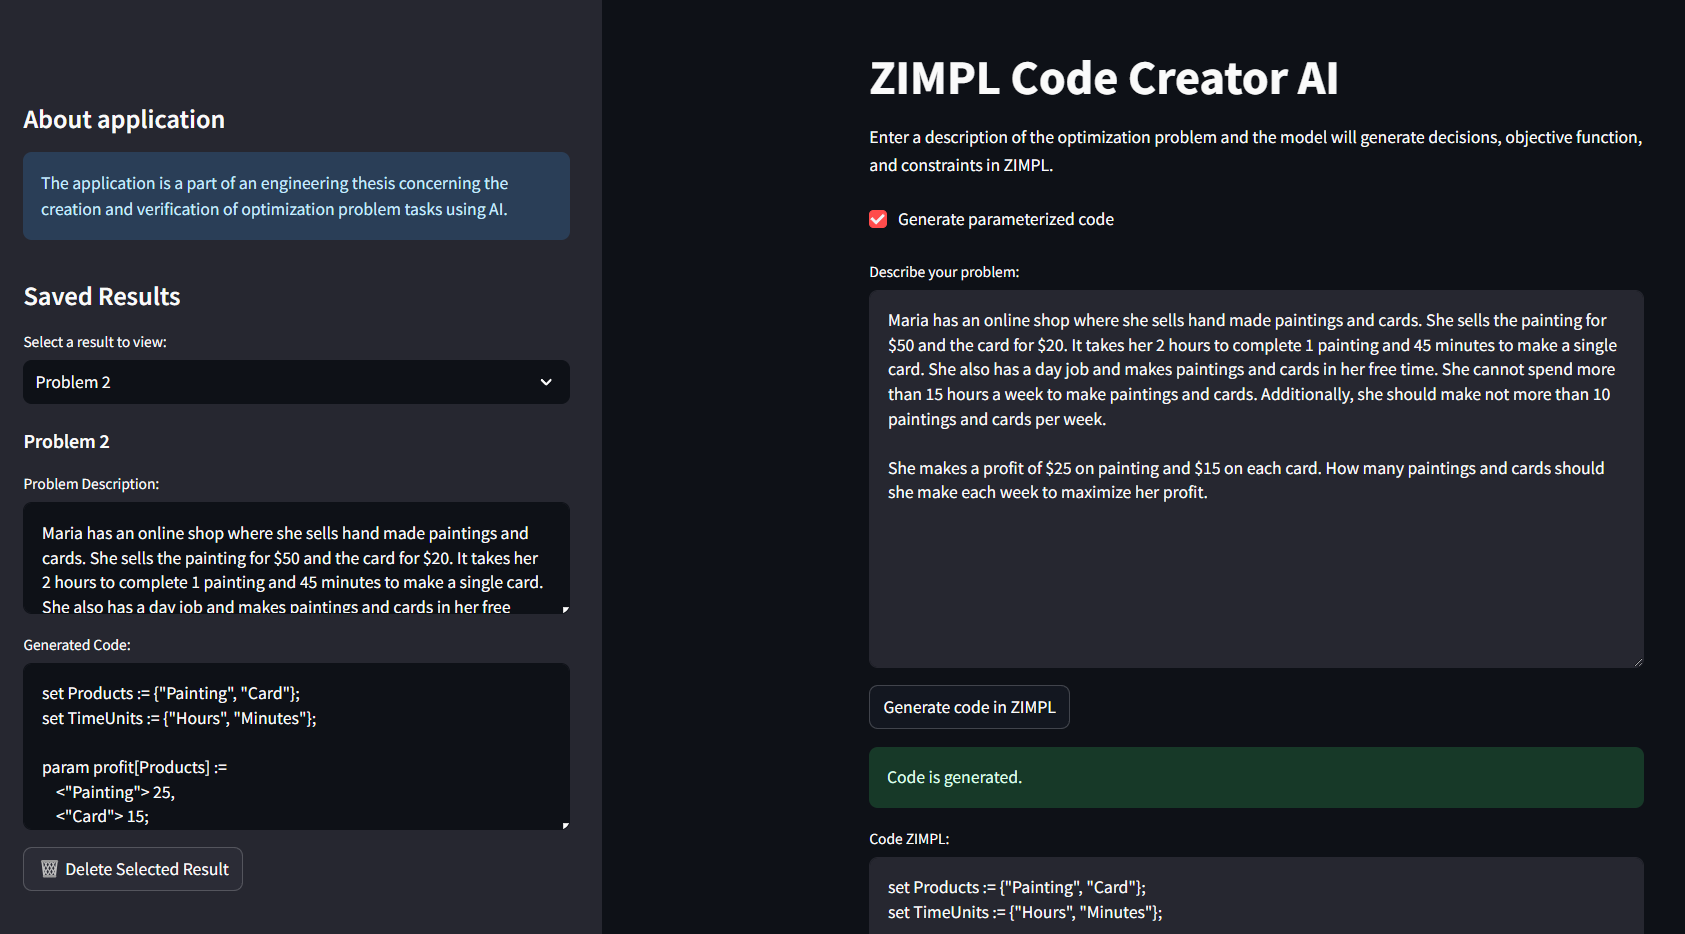
\includegraphics[width=1\linewidth]{thesis-main/figures/app.png}
    \caption{Wygląd interfejsu generatora kodu ZIMPL}
    \label{fig:gui}
\end{figure}





